% Draft paper for FIT2082: HashBoost.
%
% Every number below is taken from README.md or results/*.json. The source of
% each table is given in a `% src:` comment above it. Anything marked \todo is
% an experiment that has not been run yet, or a claim that still needs to be
% checked. Build with
%
%     latexmk -pdf paper.tex

\documentclass[a4paper, 11pt]{article}

\usepackage[margin=2.5cm]{geometry}
\usepackage{amsmath, amssymb}
\usepackage{booktabs}
\usepackage{graphicx}
\usepackage{array}
\usepackage{algorithm}
\usepackage{algpseudocode}
\usepackage{xcolor}
\usepackage{url}
\usepackage[hidelinks]{hyperref}
\usepackage[capitalise, noabbrev]{cleveref}

\newcommand{\todo}[1]{\textcolor{red}{[\textbf{TODO:} #1]}}
\newcommand{\code}[1]{\texttt{#1}}
% long \code{} names cannot hyphenate; let lines stretch instead of overflowing
\setlength{\emergencystretch}{3em}
\newcommand{\pmsd}[2]{#1\,$\pm$\,#2}

\author{Matthew Yang}
\title{Global Partitions for Boosting Time Series Classification}
\date{\today}

\begin{document}
\maketitle

% ==============================================================================
\begin{abstract}
    Gradient boosted decision trees are the usual classifier to put on top of
    interval-based time series features, but inducing each tree means searching
    for splits over the whole training set. We replace the tree with a
    \emph{global partition}: $b$ random threshold predicates, chosen from pairs
    of hard, differently labelled examples. The predicates are applied to every
    example at once and index a table of $2^b$ leaf values. The resulting
    booster, HashBoost, does no split search. It trains from mini-batches, so
    its memory use does not depend on the size of the training set. We
    implement it on the GPU in PyTorch and evaluate it after a QUANT transform
    on five MONSTER datasets and on the 112 standard UCR datasets. On UCR,
    default HashBoost is statistically level with default XGBoost (mean ranks
    2.36 and 2.39) and clearly behind QUANT's own ExtraTrees classifier (1.25).
    It beats XGBoost on small training sets and trails both on the largest. On
    MONSTER it is 0.013 to 0.083 behind the best tree ensemble, and fits in
    seconds where XGBoost takes minutes. Streaming the 975,291-row LenDB
    training pool, HashBoost's peak GPU memory is the same as at 65,536 rows
    (2.6\,GB), while XGBoost's binned matrix grows linearly to 14.6\,GB.
    HashBoost's limit is the number of rounds it can afford, not memory: every
    batch updates every existing round, so training cost is quadratic in
    rounds. Freezing old rounds makes it linear with little loss of accuracy.
\end{abstract}

\tableofcontents
\clearpage

% ==============================================================================
\section{Introduction}

Gradient boosted models are built from a sequence of decision trees, where each
tree is fitted to the residual errors of the ensemble constructed so far rather
than to the original targets~\cite{friedman2001greedy}. This stage-wise
additive formulation, together with highly engineered implementations such as
XGBoost~\cite{chen2016xgboost}, LightGBM~\cite{ke2017lightgbm} and
CatBoost~\cite{prokhorenkova2018catboost}, has made boosting the default choice
for tabular prediction tasks, where it remains competitive with, and frequently
superior to, deep learning~\cite{shwartzziv2022tabular,grinsztajn2022why}.

Boosted trees are also the usual classifier on top of interval-based time
series features. QUANT~\cite{dempster2024quant} passes its quantile features to
an ensemble of extremely randomised trees, and the features produced by
PULSAR~\cite{pulsar} and its predecessors are used the same way. At the scale
of the MONSTER benchmark~\cite{dempster2025monstermonashscalabletime}, with up
to 1.5 million series per dataset, the classifier becomes the expensive part.
Inducing a tree requires evaluating candidate split points at every node, so
each boosting iteration costs time proportional to both the number of
instances and the number of features. Histogram binning, approximate split
finding, gradient-based sampling and feature
bundling~\cite{chen2016xgboost,ke2017lightgbm,friedman2002stochastic} all
reduce the constant factor. They do not remove the need to revisit the whole
training set in every round. In practice this also means holding it in memory:
XGBoost's binned representation of LenDB after QUANT is 14.6\,GB
(\cref{sec:scaling}).

This paper asks whether the tree is needed at all. We replace each tree with a
\emph{global partition} of the feature space: $b$ axis-aligned threshold
predicates, applied to every example at once. The resulting $b$ bits index a
table of $2^b$ leaf values. The predicates are not searched for. Each one takes
a random feature and puts its threshold at the midpoint of two hard,
differently labelled examples. Each leaf value is a Newton step computed from
running sums of the gradient and hessian over the examples that land in it.
Because the partition does not depend on which examples are in the current
batch, those running sums can be updated from any later mini-batch. The model
never needs the training set in one place.

\paragraph{Contributions.}
\begin{enumerate}
    \item \textbf{HashBoost}, a gradient booster whose weak learner is a random
          global partition, and a GPU implementation that is 9.6$\times$ faster
          than the original CPU implementation and agrees with it to
          $4\times10^{-7}$ (\cref{sec:method,sec:implementation}).
    \item Two changes that make it scale. \emph{Bagging} divides the quadratic
          cost in rounds by the number of estimators. \emph{Round freezing}
          with a per-row cache turns the quadratic cost into a linear one
          (\cref{sec:freezing}).
    \item An evaluation on five MONSTER datasets against XGBoost, LightGBM and
          CatBoost (\cref{sec:accuracy}), including streamed runs over whole
          training pools of up to 1.16 million rows (\cref{sec:scaling}), and
          on the 112 standard UCR datasets against QUANT's classifier and
          XGBoost, with Friedman and Nemenyi tests (\cref{sec:ucr}).
    \item A set of negative results. Making individual partitions smarter
          (gain-based selection, feature weighting, richer features) usually
          makes the ensemble \emph{worse}, and run-to-run noise is larger than
          seeding suggests (\cref{sec:negative,sec:noise}).
\end{enumerate}

% ==============================================================================
\section{Background and Related Work}
\label{sec:related}

\paragraph{Boosting.}
Boosting originates in the observation that a set of weak learners can be
combined into an arbitrarily strong one, formalised by
AdaBoost~\cite{freund1997decision} and later generalised to arbitrary
differentiable losses as gradient boosting~\cite{friedman2001greedy}. Decision
trees are the conventional weak learner, but nothing in the gradient boosting
framework requires them. Modern implementations fit each tree to a
second-order expansion of the loss, so that a leaf's value is a Newton step
$-\sum g / \sum h$ over the examples it contains~\cite{chen2016xgboost}.
HashBoost keeps this leaf rule and changes how examples are assigned to
leaves.

\paragraph{Oblivious trees and decision tables.}
CatBoost~\cite{prokhorenkova2018catboost} grows \emph{oblivious} trees, in
which every node at a given depth uses the same split. A depth-$d$ oblivious
tree is therefore $d$ predicates whose outcomes index $2^d$ leaves. This is
the same structure as one HashBoost round, and boosted decision
tables~\cite{lou2017bdt} and neural oblivious ensembles~\cite{popov2020node}
use it too. The differences are in how the predicates are chosen and when the
leaves are fitted. CatBoost chooses each level's split greedily by gain over
the whole training set, and fixes the leaves once the tree is built. HashBoost
chooses predicates at random from a single mini-batch, and keeps
re-estimating every round's leaves as later batches arrive
(\cref{sec:method}). \todo{position more carefully against BDT: check whether
it also re-estimates leaves}

\paragraph{Randomised partitions.}
Random forests~\cite{breiman2001random} and extremely randomised
trees~\cite{geurts2006extremely} showed that much of the split search in a
tree can be replaced by randomness without losing accuracy, provided the
ensemble is large. Extremely randomised trees draw both the feature and the
threshold at random, and QUANT uses them as its
classifier~\cite{dempster2024quant}. A random global partition can also be
read as a locality-sensitive hash~\cite{indyk1998approximate}: examples that
share a code agree on $b$ random comparisons. HashBoost's thresholds are
random but not uninformed. They sit between two hard examples of different
classes, so each bit tends to separate examples the current model confuses.

\paragraph{Time series classification.}
In time series classification, random-feature methods have shown that the
expensive, data-dependent search performed by tree induction can often be
replaced by cheap, data-independent random transformations.
ROCKET~\cite{dempster2020rocket} applies a large bank of random convolutional
kernels followed by a linear classifier. It achieves accuracy comparable to far
more expensive ensembles such as HIVE-COTE~\cite{middlehurst2021hivecote2} at a
small fraction of the training cost. MiniRocket~\cite{dempster2021minirocket}
and Hydra~\cite{dempster2023hydra} refine this approach further. A parallel
line of work extracts features from intervals of the series. Time Series
Forest~\cite{deng2013tsf} computes simple summary statistics over randomly
selected intervals and passes them to a tree ensemble. The idea was developed
further in CIF~\cite{middlehurst2020cif}, DrCIF~\cite{middlehurst2021hivecote2},
rSTSF~\cite{cabello2021rstsf}, QUANT~\cite{dempster2024quant} and
PULSAR~\cite{pulsar}. All of these end in some form of tree. We use QUANT and
PULSAR as fixed feature transforms and replace only the classifier.

% ==============================================================================
\section{Method}
\label{sec:method}

\subsection{A round is a global partition}

Let $x \in \mathbb{R}^p$ be a feature vector and $k$ the number of classes. A
round $r$ is defined by $b$ pairs $(j_{r,i}, t_{r,i})$ of a feature index and a
threshold, for $i = 0, \dots, b-1$. It maps $x$ to a $b$-bit code
\begin{equation}
    c_r(x) = \sum_{i=0}^{b-1} 2^i \, \mathbb{1}\!\left[x_{j_{r,i}} \le t_{r,i}\right]
    \in \{0, \dots, 2^b - 1\},
\end{equation}
and has a table $L_r \in \mathbb{R}^{2^b \times k}$ of leaf values. The model
after $R$ rounds is
\begin{equation}
    F(x) = \sum_{r=1}^{R} L_r\!\left[c_r(x)\right] \in \mathbb{R}^k,
\end{equation}
and predicts $\mathrm{softmax}(F(x))$. We use $b = 8$ throughout, so each round
has 256 buckets. A round is an oblivious tree of depth 8 with every split
fixed in advance.

\subsection{Choosing the predicates}

Given the current batch, its probabilities and its labels, a new round's
predicates are chosen as follows (\code{HardPairSplitter}):
\begin{enumerate}
    \item Order the batch by cross entropy, hardest first.
    \item Walk that order and greedily form $b$ pairs of examples with
          different labels.
    \item For each pair $(u, v)$, draw a feature $j$ uniformly at random and set
          $t = (u_j + v_j)/2$.
\end{enumerate}
Each bit therefore separates two examples the model currently gets wrong, and
the only search is the sort in the first step. The \emph{sampled} variant
replaces the strict ordering with successive draws without replacement,
proportional to cross entropy, using the Gumbel-top-$k$
trick~\cite{kool2019stochastic}. The strict ordering keeps pairing the same
dozen persistent outliers each time a batch comes round, and sampling spreads
the pairs across the hard end of the batch.

\subsection{Fitting the leaves}

We use the softmax cross-entropy gradient $g = p - \mathrm{onehot}(y)$ and a
floored diagonal hessian $h = p(1-p) + 10^{-3}$. Every round keeps running sums
$G_r, H_r \in \mathbb{R}^{2^b \times k}$ of $-g$ and $h$ over the examples that
landed in each bucket, and its leaf values are
\begin{equation}
    L_r[s] = \eta \, \frac{G_r[s]}{H_r[s] + \epsilon},
\end{equation}
with learning rate $\eta = 0.1$ and $\epsilon = 10^{-6}$.

The key departure from tree boosting is \emph{when} these sums are
accumulated. A tree's leaves are fitted once, when the tree is built, and
never change. In HashBoost, \textbf{every mini-batch is accumulated into every
existing round}, with gradients evaluated at the current model
(\cref{alg:hashboost}). A round created early keeps absorbing evidence from
every batch that follows. This is what lets the model learn from a stream,
since a round is not tied to the batch that created it. It resembles
backfitting of additive models~\cite{buja1989linear}, applied online.
It is also where the cost comes from: a batch costs $O(R)$ once there are $R$
rounds, so $T$ batches with one new round each cost $O(T^2)$.

\begin{algorithm}[t]
    \caption{One HashBoost step on a mini-batch $(X, y)$ of $n$ examples. The
        default adds $H = 1$ round per batch.}
    \label{alg:hashboost}
    \begin{algorithmic}[1]
        \For{$h = 1, \dots, H$}
        \State $F \gets \sum_{r < R} L_r[c_r(X)]$ \Comment{$(n, k)$ logits}
        \State $p \gets \mathrm{softmax}(F)$;\quad $g \gets p - \mathrm{onehot}(y)$;\quad $h \gets p(1-p) + 10^{-3}$
        \State choose predicates of round $R$ from hard pairs in $(X, y, p)$
        \For{$r = 0, \dots, R$} \Comment{all rounds, including the new one}
        \State $G_r[c_r(X)] \mathrel{+}= -g$;\quad $H_r[c_r(X)] \mathrel{+}= h$ \Comment{scatter-add}
        \State $L_r \gets \eta\, G_r / (H_r + \epsilon)$
        \EndFor
        \State $R \gets R + 1$
        \EndFor
    \end{algorithmic}
\end{algorithm}

\subsection{Extensions}
\label{sec:extensions}

All of the following are opt-in. The defaults reproduce the algorithm above,
which is checked against an independent reference implementation
(\cref{sec:implementation}).

\paragraph{Capacity ($H$ rounds per batch).}
\code{hashes\_per\_round}$\,=H$ adds $H$ rounds per batch instead of one, which
raises capacity without more passes over the data. Because each of the $H$
steps re-accumulates the batch into the existing rounds, it also weights each
batch $H$ times in old rounds. A variant that added two rounds but updated old
rounds only once lost most of the gain on Pedestrian (0.2301 against 0.2122).

\paragraph{Bagging.}
\code{BaggedHashBoost} averages the logits of $E$ independent models, each
trained on the full data with its own random draws. Cost is quadratic in rounds
\emph{per model}, so $E$ models of $R/E$ rounds cost $R^2/E$ against $R^2$ for
one deep model.

\paragraph{Round freezing.}
\label{sec:freezing}
With \code{active\_rounds}$\,=W$, only the newest $W$ rounds keep
accumulating. Older rounds are frozen, and a frozen round's contribution to a
given example never changes again. Given stable row ids, each row's frozen
contribution is summed once, cached in an $(N, k)$ table, and never recomputed.
A batch then costs $O(W + f)$, where $f$ is the number of rounds frozen since
its rows were last seen, so the total cost becomes linear in rounds. In experiments $W$ is set in epochs
(\code{frozen\_10ep} keeps ten epochs' worth of rounds active).

\paragraph{Refitted readout.}
Each leaf is a Newton step computed as if every other round were fixed. After
boosting, the tables can instead be fitted \emph{jointly}. $L$ has shape $(R,
2^b, k)$, the same as a multiclass linear model on one-hot codes, so we warm
start from the boosted values and run Adam on cross entropy with a penalty
toward the boosted solution, early-stopping on a separate tune slice. Three
parameterisations are compared: one gain per round (\code{round}), one per
(round, class) (\code{round\_class}), and the full table (\code{table}).

\paragraph{Mass-adaptive leaf smoothing.}
Most buckets are empty (about 203 of 256 on Pedestrian), and an empty bucket
contributes nothing. \code{shrinkage\_tau} mixes each bucket's statistics with
the mean of its $b$ Hamming neighbours, which differ from it by exactly one
predicate, with weight $\alpha_s = \tau/(\tau + \sum_k H_r[s,k])$. An empty
bucket takes its neighbours' evidence in full, while a well-populated one is
left almost unchanged.

\subsection{Implementation}
\label{sec:implementation}

HashBoost runs entirely on the GPU in PyTorch. Three layout decisions carry
most of the performance:
\begin{itemize}
    \item \textbf{Codes are round-major and one byte each.} A batch's codes
          are a \code{uint8} tensor of shape $(R, n)$, built one bit at a time
          so the largest intermediate is a single gather. With
          \code{torch.compile}, each bit becomes one fused kernel.
    \item \textbf{Gradient and hessian are fused.} $G$ and $H$ share one
          $(R, 2^b, 2k)$ tensor, so a single \code{scatter\_add\_} over an
          expanded view updates both, without materialising the per-round
          copy.
    \item \textbf{Work is chunked over rounds} to a fixed memory budget, so
          peak memory does not grow with $R$ beyond the tables themselves.
\end{itemize}
The original implementation, a numba CPU loop, is kept as a reference. Given
the same predicates, the two agree to $4\times10^{-7}$ in logits with identical
argmax, and a test suite enforces that the defaults stay equal to it. On
Pedestrian (800 rounds, 50 epochs) the GPU version cut training from 101.5\,s
to 10.6\,s. Later kernel changes reduced it to about 7.5\,s, with identical
results (\cref{tab:kernels}).

% src: README "hashboost-screen" > "Exact kernels" (cf658bc)
\begin{table}[t]
    \centering
    \caption{Kernel changes on Pedestrian, 800 rounds (\code{baseline}) and
        1600 rounds (\code{capacity\_2}). Results are identical. Compilation
        costs about 5.5\,s on first use.}
    \label{tab:kernels}
    \begin{tabular}{lrrrr}
        \toprule
        variant              & before & eager  & compiled     & peak GPU (MB)          \\
        \midrule
        \code{baseline}      & 11.4\,s & 8.9\,s  & $\sim$7.5\,s & 428 $\to$ 284 \\
        \code{capacity\_2}   & 38.5\,s & 26.7\,s & 24.9\,s      & 771 $\to$ 491 \\
        \bottomrule
    \end{tabular}
\end{table}

% ==============================================================================
\section{Experimental Setup}
\label{sec:setup}

\paragraph{Datasets.}
We use five datasets from MONSTER~\cite{dempster2025monstermonashscalabletime}
(\cref{tab:datasets}). MONSTER supplies fixed cross-validation folds, and we
hold out fold 0 as the test set throughout.

% src: data/*.npy shapes; QUANT feature counts from results/*.json;
%      PULSAR counts from README "pulsar".
\begin{table}[t]
    \centering
    \caption{Datasets. ``Pool'' is the number of rows outside test fold 0.}
    \label{tab:datasets}
    \begin{tabular}{lrrrrrr}
        \toprule
        dataset     & series    & pool      & channels & length & classes & QUANT features \\
        \midrule
        Pedestrian  & 189,621   & 151,696   & 1        & 24     & 82      & 212            \\
        InsectSound & 50,000    & 40,000    & 1        & 600    & 10      & 5,470          \\
        LenDB       & 1,244,942 & 983,483   & 3        & 540    & 2       & 14,940         \\
        Tiselac     & 99,687    & 79,907    & 10       & 23     & 9       & 2,040          \\
        Traffic     & 1,460,968 & 1,168,774 & 1        & 24     & 7       & 212            \\
        \bottomrule
    \end{tabular}
\end{table}

\paragraph{Splits.}
Unless stated otherwise, models are trained on 65,536 rows drawn from the pool
by a fixed shuffle (seed 42). InsectSound uses 32,768, because its pool is too
small for 65,536 plus the evaluation slices. The next 4,096 rows are the
validation set and the 4,096 after that are a tune slice, used only for
decisions made after training (early stopping of the readout). Streamed runs
(\cref{sec:scaling}) train on the whole pool, and hold the same validation rows
as the 65,536-row runs they are compared to. Every comparison between HashBoost
and a tree model on MONSTER uses these same training and validation rows.

The exploratory Pedestrian sweeps (\cref{tab:ladder,tab:frozen,tab:tau}) and
the QUANT/PULSAR comparison were run earlier, on a different shuffle (seed 123).
They are compared only with each other, except where \cref{tab:ladder} sets
them beside XGBoost, and that one comparison crosses the two splits. With 4,096
validation rows, the binomial standard error at 20\% error is
$\sqrt{0.2 \cdot 0.8/4096} \approx 0.006$, so a gap under $\sim$0.01 across the
splits is not a result.

\paragraph{UCR.}
We also use the 112 univariate UCR datasets~\cite{dau2019ucr} with equal
lengths and no missing values, the set the bake-off reports
on~\cite{middlehurst2024bakeoff}. These are the archive's 128 datasets less
the 15 with missing values or variable lengths, and less Fungi, which has one
training series per class. Each dataset uses the archive's default train/test
split. The training sets are small: they range from 16 to 8,926 series (median
190), 27 have 50 or fewer, and only 11 have 1,000 or more. Lengths range from
15 to 2,844 and class counts from 2 to 60. UCR has no validation split, so
every model runs at fixed settings, nothing is chosen after training, and we
report test error.

\paragraph{Features.}
QUANT~\cite{dempster2024quant} (depth 6, $\mathrm{div}=4$) is fitted on the
first training batch, and is the transform used for every result unless stated
otherwise. PULSAR~\cite{pulsar} is supervised, and its Fisher-score selection
is fitted on the training rows alone. Both are our PyTorch ports. The PULSAR
port matches upstream's feature counts exactly and its global features to
$10^{-4}$. About 0.5\% of its local features differ, all at ties.

\paragraph{Baselines.}
XGBoost (GPU \code{hist}, depth 6), LightGBM (31 leaves) and CatBoost (GPU,
depth 6), all with learning rate 0.05, up to 1,000 rounds and early stopping
after 50 rounds without improvement. A single unpruned decision tree is included
as a floor. \todo{Tree-model figures are the best point on the validation
curve, i.e.\ selected on validation. HashBoost figures are the final error.
This flatters the trees, but it should still be made consistent, e.g.\ by
early-stopping on the tune slice.}

On UCR, where there is nothing to early-stop on, the baselines are
ExtraTrees with QUANT's own settings (200 trees, entropy criterion, a tenth of
the features per split)~\cite{dempster2024quant}, on the same QUANT features
as HashBoost, and XGBoost at its library defaults (100 rounds, learning rate
0.3, depth 6).

\paragraph{HashBoost defaults.}
$b=8$, $\eta=0.1$, batch size 4,096, 50 epochs. For 65,536 rows that is 16
batches per epoch and 800 rounds. Most UCR training sets fit in a single batch,
where 50 epochs would mean 50 rounds. On UCR the budget is therefore 800 rounds
of the same model: batches of at most 4,096 rows, cycled until 800 rounds
have been added.

\paragraph{Hardware.}
One NVIDIA RTX 4060 (8\,GB) with 7.9\,GB of host RAM under WSL2. The memory
limits shaped much of the design. For example, a 3,200-round single model
peaked near the card's limit.

\paragraph{Measurement protocol.}
\label{sec:noise-protocol}
We report validation misclassification error. Every variant is compared with a
baseline rerun \emph{in the same sweep}. Differences under about 0.006 on
Pedestrian are not treated as results, for the reasons in \cref{sec:noise}.
Where a change does not alter training (the readout), the comparison is paired
against the same fitted model. Unless stated, results are the mean $\pm$
standard deviation over 3 runs.

% ==============================================================================
\section{Results}

\subsection{Accuracy against tree ensembles (RQ1, RQ3)}
\label{sec:accuracy}

\Cref{tab:baselines} compares \emph{default} HashBoost (a single model, 50
epochs: 800 rounds, or 400 on InsectSound's 32,768 rows) with the tree
ensembles, all on the same rows.
HashBoost trails the best tree model on every dataset. The gap ranges from
0.013 on LenDB to 0.083 on InsectSound. HashBoost fits in 3--14\,s on the GPU.
Pedestrian ran first, so its figure includes a one-off compilation of about
5\,s. XGBoost took 333\,s on Pedestrian. Among the trees, the winner changes: XGBoost is best on
Pedestrian, InsectSound and LenDB, and LightGBM on Tiselac and Traffic.
CatBoost, whose oblivious trees are structurally closest to HashBoost, is worse
than default HashBoost on Pedestrian and Tiselac. On Traffic it lies between
HashBoost and the other two tree models.

% src: tree models: results/{Pedestrian-4eb8d6b, InsectSound-45dfeb7,
%      LenDB-6205faa, Tiselac-4ec0c0d, Traffic-80864c4}.json, min of the
%      validation curve. HashBoost: results/{D}-sweep-f1cfcef.json, experiment.py
%      --variants baseline --seeds 1 at the seed-42 split, final error.
\begin{table}[t]
    \centering
    \caption{Validation error, 65,536 training rows (InsectSound 32,768),
        QUANT features, one run each, all on the seed-42 split. HashBoost is the
        default single model at its final round. The trees are at the best
        point on their validation curves. LightGBM diverged on Pedestrian (final
        error 0.896). The gap is to the best tree model. --: not run. An earlier
        run of default HashBoost on the same Pedestrian rows read 0.2253.}
    \label{tab:baselines}
    \begin{tabular}{lrrrrrrr}
        \toprule
        dataset     & HashBoost & fit     & XGBoost         & LightGBM        & CatBoost & tree   & gap    \\
        \midrule
        Pedestrian  & 0.2356    & 13.9\,s & \textbf{0.2041} & 0.2849$^\ast$   & 0.2427   & 0.4397 & +0.032 \\
        InsectSound & 0.2712    & 4.0\,s  & \textbf{0.1887} & --              & --       & --     & +0.083 \\
        LenDB       & 0.0591    & 8.6\,s  & \textbf{0.0459} & --              & --       & --     & +0.013 \\
        Tiselac     & 0.0818    & 4.0\,s  & 0.0659          & \textbf{0.0632} & 0.0928   & 0.1650 & +0.019 \\
        Traffic     & 0.4365    & 3.4\,s  & 0.3989          & \textbf{0.3936} & 0.4226   & 0.5310 & +0.043 \\
        \bottomrule
    \end{tabular}
\end{table}

\todo{Still needed for \cref{tab:baselines}: (a) LightGBM and CatBoost on InsectSound
and LenDB, (b) tree timings measured the same way as HashBoost's, (c) several
runs per cell (Pedestrian's two runs of default HashBoost read 0.2253 and
0.2356), (d) the trees early-stopped on the tune slice rather than selected on
validation, and (e) test-fold error, evaluated once after everything is
frozen. See \cref{sec:todo}.}

\paragraph{Closing the gap on Pedestrian.}
Pedestrian received the most tuning. \Cref{tab:ladder} shows the path from the
default to XGBoost's level. Two things stand out. Capacity helps more than
averaging at equal hash count (\code{capacity\_2} 0.2150 against two bagged
800-round models 0.2204). But bagging is far cheaper per hash, and combining
the two is best. At 3,200 hashes, four 800-round models take 43.5\,s where one
3,200-round model takes 818\,s. \code{bagged\_4\_capacity\_2} matches XGBoost
at less than half its training time. Refitting its readout jointly takes it to
0.2006, the first HashBoost result below XGBoost's 0.2041. These sweeps
used the earlier split, however, so that comparison crosses splits and a
gap of 0.0035 is not a result (\cref{sec:setup}).

% src: README cac8e0b, b21d3e8, 3d25491. Each row was measured in a
%      different sweep; see the caption.
\begin{table}[t]
    \centering
    \caption{Pedestrian, seed-123 split, 3 runs each. Rows come from
        different sweeps, whose baselines ranged from 0.2214 to 0.2270
        (\cref{sec:noise}), so differences between adjacent rows under
        $\sim$0.006 are not meaningful. The XGBoost figure is from the seed-42
        split, so that comparison crosses splits (\cref{sec:setup}).}
    \label{tab:ladder}
    \begin{tabular}{lrrr}
        \toprule
        model                                                & hashes & val error                  & wall    \\
        \midrule
        \code{baseline}                                      & 800    & \pmsd{0.2240}{0.0004}      & 10.5\,s \\
        \code{bagged\_4} (4 $\times$ 800)                    & 3,200  & \pmsd{0.2128}{0.0024}      & 43.5\,s \\
        \code{capacity\_4} (1 $\times$ 3,200)                & 3,200  & \pmsd{0.2103}{0.0012}      & 818\,s  \\
        \code{bagged\_4\_capacity\_2} (4 $\times$ 1,600)     & 6,400  & \pmsd{0.2059}{0.0017}      & 148\,s  \\
        \quad + \code{round\_class} readout                  & 6,400  & \pmsd{\textbf{0.2006}}{0.0025} & 375\,s \\
        \midrule
        XGBoost (best point on curve)                        &        & 0.2041                     & 333\,s  \\
        \bottomrule
    \end{tabular}
\end{table}

\paragraph{Feature transform.}
The largest single gain we measured came from the features, not the model.
Replacing QUANT with PULSAR reduced InsectSound's error from
\pmsd{0.2699}{0.0094} to \pmsd{0.2262}{0.0044} (3 runs, same rows), about half
the gap to XGBoost on QUANT. It \emph{increased} Pedestrian's from
\pmsd{0.2326}{0.0059} to \pmsd{0.2481}{0.0034}. On whole-pool Traffic the two
were level (0.3895 against 0.3931, one run each), with PULSAR taking twice the
wall time. One untested explanation for Pedestrian is dilution. HashBoost
draws features uniformly, and PULSAR offers 3,000 columns where QUANT offers
212. \todo{XGBoost on PULSAR features, to separate the transform's effect from
its interaction with HashBoost.}

\subsection{The UCR archive (RQ3)}
\label{sec:ucr}

\Cref{tab:ucr} summarises default HashBoost, ExtraTrees and XGBoost on the
UCR 112, each dataset on its default split and run once. First, a check on the
pipeline: our ExtraTrees reproduces the published QUANT results on the same
splits~\cite{middlehurst2024bakeoff}. Its mean error is 0.1475 against 0.1456,
the correlation across datasets is 0.996, and the 12 datasets that differ by
more than 0.02 split six each way.

% src: notebooks/ucr.ipynb, over results/UCR/*-84ac59c.json; the published
%      rows are resample 0 of the bake-off's QUANT and HC2 result files.
\begin{table}[t]
    \centering
    \caption{UCR 112: test error on the default splits, one run per dataset.
        Mean rank is among the three models we ran (1 is the lowest error).
        W/T/L is HashBoost's record against each row: the datasets where its
        error is lower, equal and higher. Total fit is summed over the 112. $p$ is a two-sided Wilcoxon
        signed-rank test against HashBoost, Holm-adjusted over the four
        comparisons. The published rows are the bake-off's resample 0, which is
        the default split, and are shown for reference.}
    \label{tab:ucr}
    \small
    \setlength{\tabcolsep}{5pt}
    \begin{tabular}{lrrrrrr}
        \toprule
        model             & mean error      & median & mean rank     & W/T/L           & $p$                 & total fit    \\
        \midrule
        HashBoost         & 0.1941          & 0.1705 & 2.36          & --              & --                  & 183\,s       \\
        ExtraTrees        & \textbf{0.1475} & 0.1205 & \textbf{1.25} & 8/8/96          & $2.6\times10^{-14}$ & 70\,s        \\
        XGBoost           & 0.2101          & 0.1912 & 2.39          & 58/3/51         & 0.082               & 413\,s       \\
        \midrule
        QUANT (published) & 0.1456          & 0.1177 &               & 13/5/94         & $4.9\times10^{-14}$ &              \\
        HC2 (published)   & 0.1236          & 0.0753 &               & 8/7/97          & $3.8\times10^{-15}$ &              \\
        \bottomrule
    \end{tabular}
\end{table}

\begin{figure}[t]
    \centering
    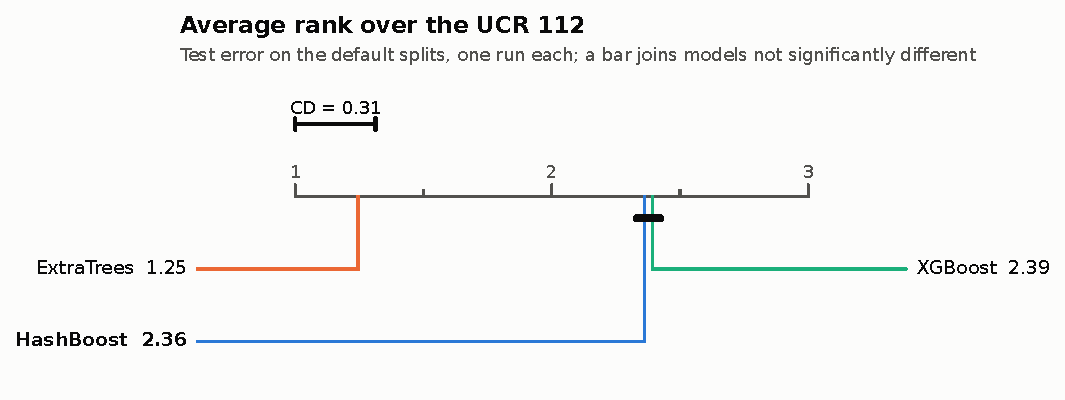
\includegraphics[width=0.85\linewidth]{figures/ucr_cd.pdf}
    \caption{Critical difference diagram over the UCR
        112~\cite{demsar2006statistical}. A Friedman test rejects equal ranks
        ($p = 3.6\times10^{-22}$). A bar joins models that are within the Nemenyi
        critical difference (0.31) of each other at $\alpha = 0.05$.}
    \label{fig:ucr-cd}
\end{figure}

A Friedman test rejects equal performance across the three models
($p = 3.6\times10^{-22}$), and the Nemenyi test splits them into two groups
(\cref{fig:ucr-cd}). ExtraTrees is significantly better than both boosters.
HashBoost and XGBoost are not significantly different: their mean ranks are
2.36 and 2.39, and HashBoost has the lower error on 58 datasets and the higher
on 51. Against ExtraTrees, HashBoost has the lower error on only 8.

The record against XGBoost depends on the size of the training set
(\cref{tab:ucr-bands}). HashBoost's lead over XGBoost comes entirely from the
58 datasets with at most 200 training rows, where XGBoost's defaults do badly.
There HashBoost wins 39 and loses 17. Above 200 rows it wins 19 and loses 34.
On the 11 datasets with at least 1,000 rows it trails both baselines
(Holm-adjusted $p$ of 0.012 against ExtraTrees and 0.032 against XGBoost).
Against ExtraTrees it loses in every band (\cref{fig:ucr-scatter}). The gap to
ExtraTrees correlates more with the number of classes ($r = 0.31$) than with
training size ($r = -0.11$). Three of the five widest gaps are the Pig datasets,
which have 52 classes and two training series per class.

% src: notebooks/ucr.ipynb, the size-band cell
\begin{table}[t]
    \centering
    \caption{UCR 112 by training-set size: HashBoost's W/T/L against each
        baseline, and each model's mean test error.}
    \label{tab:ucr-bands}
    \small
    \setlength{\tabcolsep}{5pt}
    \begin{tabular}{lrrrrrr}
        \toprule
        training rows & datasets & vs ExtraTrees & vs XGBoost & HashBoost & ExtraTrees & XGBoost \\
        \midrule
        $\le 50$      & 27       & 3/0/24        & 19/1/7     & 0.1141    & 0.0646     & 0.1841  \\
        51--200       & 31       & 2/4/25        & 20/1/10    & 0.1981    & 0.1404     & 0.2198  \\
        201--999      & 43       & 2/4/37        & 16/1/26    & 0.2598    & 0.2176     & 0.2461  \\
        $\ge 1000$    & 11       & 1/0/10        & 3/0/8      & 0.1225    & 0.0973     & 0.1054  \\
        \bottomrule
    \end{tabular}
\end{table}

\begin{figure}[t]
    \centering
    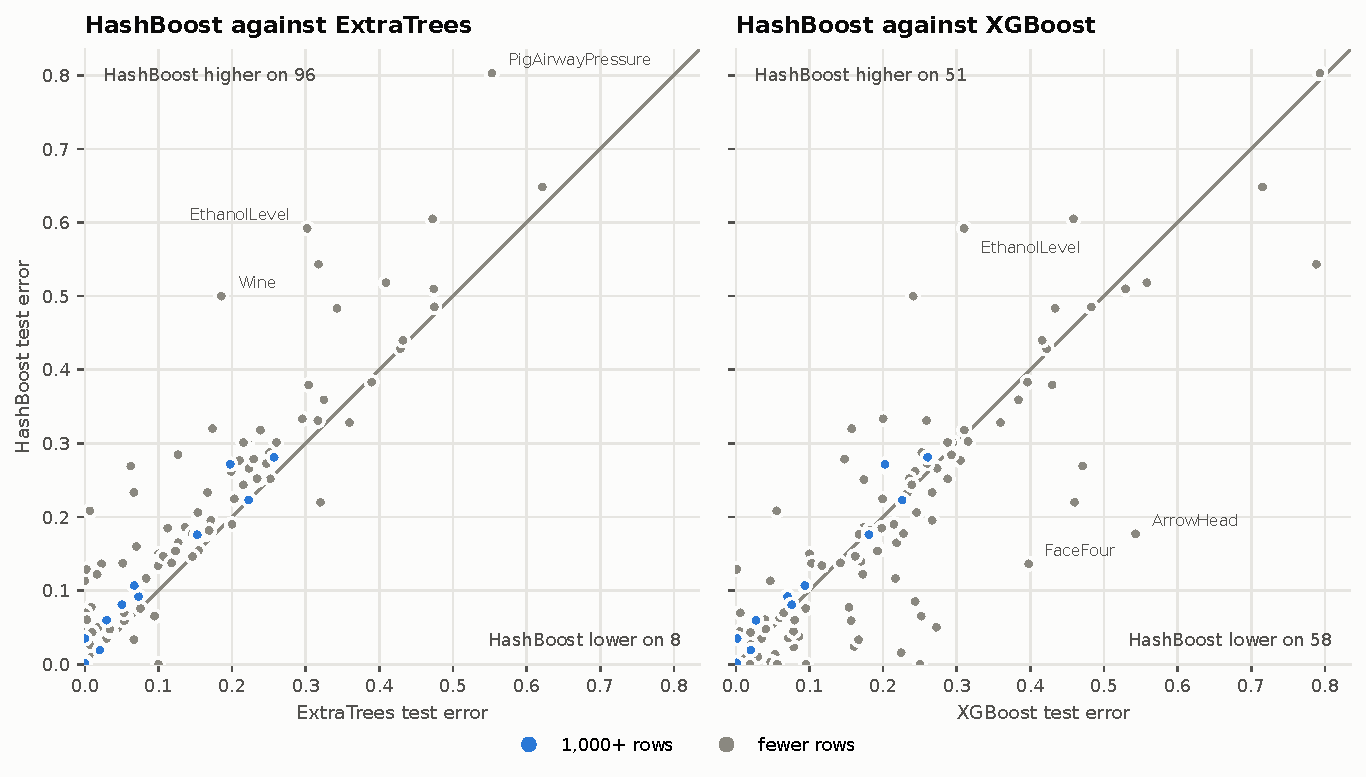
\includegraphics[width=\linewidth]{figures/ucr_scatter.pdf}
    \caption{HashBoost's test error against each baseline's, one point per UCR
        dataset. Below the diagonal, HashBoost has the lower error. Blue marks
        the 11 datasets with at least 1,000 training rows.}
    \label{fig:ucr-scatter}
\end{figure}

Cost follows from the fixed budget. HashBoost fits every dataset in
1.4--2.8\,s (median 1.6\,s). A training set that fits in one batch is
re-accumulated every round, so the time hardly depends on the data.
ExtraTrees fits most small datasets in 0.2\,s on the CPU. On the 11 largest
datasets HashBoost is the fastest in total (24\,s, against 37\,s for ExtraTrees
and 101\,s for XGBoost), but it is also the least accurate there. The budget is
not a ceiling. HashBoost reaches zero training error on 111 of the 112
datasets, yet its mean test error keeps falling, from 0.202 at 400 rounds to
0.194 at 800. This was recorded for plotting only, and nothing was chosen on it.

\subsection{Training cost and scaling with instances (RQ2)}
\label{sec:scaling}

\paragraph{Cost is quadratic in rounds.}
Every batch updates every round, so per-batch cost grows linearly with the
number of rounds. On a streamed Traffic run it rose from 2\,ms to 14.5\,ms per
batch over 2,840 rounds. Total training cost is therefore quadratic: 1,600
rounds took 37.5\,s against 10.5\,s for 800. Where the time goes depends on the
dataset (\cref{tab:profile}). Many classes make the scatter-add dominate, and
many features make encoding dominate.

% src: README "hashboost-screen" > "Where the time goes"
\begin{table}[t]
    \centering
    \caption{Share of one training batch by stage.}
    \label{tab:profile}
    \begin{tabular}{lrrr}
        \toprule
                                   & Pedestrian & InsectSound & LenDB    \\
        \midrule
        features / classes         & 212 / 82   & 5,470 / 10  & 14,940 / 2 \\
        ms per batch (at rounds)   & 27.9 (800) & 13.5 (800)  & 18.3 (1,200) \\
        accumulate                 & 57\%       & 21\%        & 8\%      \\
        encode                     & 19\%       & 43\%        & 47\%     \\
        predict                    & 10\%       & 11\%        & 10\%     \\
        refresh leaves             & 10\%       & 3\%         & 1\%      \\
        transpose                  & 1\%        & 14\%        & 28\%     \\
        objective + propose        & 4\%        & 9\%         & 7\%      \\
        \bottomrule
    \end{tabular}
\end{table}

\paragraph{Freezing makes it linear.}
\Cref{tab:frozen} shows round freezing on Pedestrian. A 10-epoch window
reproduces \code{capacity\_2}'s accuracy in 2.4$\times$ less time. A second
sweep repeated this (0.2129 in 10.3\,s against 0.2137 in 24.7\,s). The window
is a real hyperparameter. On Pedestrian a 2-epoch window cost between +0.008
and +0.027 across four sweeps. On InsectSound even 2 epochs cost nothing
measurable. On streamed whole-pool runs a 2-epoch window also cost nothing
measurable, on Traffic (0.3877 against 0.3922) and on LenDB (0.0751 against
0.0745). Freezing held Traffic's per-batch model cost near 7.5\,ms instead of
letting it grow.

% src: README "hashboost-screen" > "Frozen rounds" (d39acad)
\begin{table}[t]
    \centering
    \caption{Round freezing on Pedestrian, 3 runs, one sweep, compiled.}
    \label{tab:frozen}
    \begin{tabular}{lrr}
        \toprule
        variant                            & val error                          & wall            \\
        \midrule
        \code{baseline} (800 rounds)       & \pmsd{0.2252}{0.0023}              & 8.4\,s          \\
        \code{frozen\_10ep}                & \pmsd{0.2276}{0.0037}              & 3.6\,s          \\
        \code{frozen\_2ep}                 & \pmsd{0.2332}{0.0042}              & 1.8\,s          \\
        \code{capacity\_2} (1,600 rounds)  & \pmsd{0.2133}{0.0025}              & 25.6\,s         \\
        \code{frozen\_10ep\_capacity\_2}   & \pmsd{\textbf{0.2135}}{0.0032}     & \textbf{10.8\,s} \\
        \bottomrule
    \end{tabular}
\end{table}

\paragraph{Memory does not grow with the training set.}
\Cref{tab:streaming} streams the whole LenDB training pool, 975,291 rows, and
compares it with the 65,536-row runs on the same validation rows. The pool is
6.3\,GB as raw series, more than the host can hold alongside anything else,
and 58\,GB after QUANT. Neither model materialises the features.
HashBoost's peak GPU memory was \emph{identical} at both sizes, 2,572\,MB,
because each batch is folded into the tables and freed. XGBoost's binned
matrix (the ellpack) is almost exactly one byte per element and grows linearly
with rows (\cref{tab:ellpack}). At the full pool it pages 14.6\,GB from disk
every round, at 171$\times$ the in-memory cost per round. Reaching the 179
rounds of the 65,536-row run would have taken about six hours.

% src: README "streaming-baselines"
\begin{table}[t]
    \centering
    \caption{LenDB, streamed. One run each.}
    \label{tab:streaming}
    \begin{tabular}{lrrrrrr}
        \toprule
        model     & rows    & rounds & train  & val             & wall   & peak GPU \\
        \midrule
        HashBoost & 65,536  & 1,200  & 0.0049 & 0.0532          & 230\,s & 2,572\,MB \\
        HashBoost & 975,291 & 1,195  & 0.0608 & 0.0691          & 560\,s & 2,572\,MB \\
        XGBoost   & 65,536  & 179    & 0.0236 & \textbf{0.0459} & 131\,s & 6,223\,MB \\
        XGBoost   & 975,291 & 3      & 0.0566 & 0.0627          & 702\,s & 6,021\,MB \\
        \bottomrule
    \end{tabular}
\end{table}

\begin{table}[t]
    \centering
    \caption{XGBoost's external-memory ellpack on LenDB grows linearly with
        rows, and so does its per-round cost.}
    \label{tab:ellpack}
    \begin{tabular}{rrr}
        \toprule
        rows    & ellpack    & s/round \\
        \midrule
        65,536  & in RAM     & 0.68    \\
        122,880 & 1.8\,GB    & 8.9     \\
        245,760 & 3.7\,GB    & 16.2    \\
        975,291 & 14.6\,GB   & 116.0   \\
        \bottomrule
    \end{tabular}
\end{table}

\paragraph{More data needs more rounds.}
At the same number of rounds, the 65,536-row model is \emph{better} than the
full-pool model (0.0532 against 0.0691). The training errors explain it. The
small model has memorised its training set (0.0049), while the full-pool model
sits at 0.0608 against 0.0691 on validation, which is underfitting. About 1,200
rounds are enough to memorise 65,536 rows and nowhere near enough for 975,291,
and the full-pool curve was still descending when the run stopped. HashBoost's
scaling is limited by compute in rounds, not by memory, and the quadratic cost
is what makes rounds expensive.

On Traffic, where the full pool is 1.16 million rows, whole-pool training does
pay. From 65,536 rows HashBoost scored 0.4404 against XGBoost's 0.3997 and
LightGBM's 0.3950. Ten streamed epochs over the whole pool (2,840 rounds)
reached 0.3922 unfrozen and 0.3877 with a 2-epoch window, level with the tree
models trained on 65,536 rows, in 139--154\,s. In these streamed runs the model
was only 14--19\% of wall time on Traffic and under 4\% on LenDB. Most of the
time went to the QUANT transform and to reading the memory-mapped input.

\todo{The decisive RQ2 experiment: whole-pool LenDB with freezing and enough
epochs to stop underfitting (e.g.\ 20--50 epochs, 2-epoch window). Does
HashBoost then beat both its own 65,536-row run and XGBoost at 65,536 rows,
within the same 2.6\,GB?}

\todo{A figure: validation error against wall time (or rounds) for HashBoost
and XGBoost at 65k and full pool. The data is in results/LenDB-full-*.json and
results/Traffic-full-*.json. notebooks/streaming.ipynb may already plot it.}

\subsection{What did not work}
\label{sec:negative}

\paragraph{Smarter partitions make a worse ensemble.}
Choosing each round's predicates as the best of $K$ candidates by boosting gain
raised the number of occupied buckets from 79 to 119 of 256, and made the
ensemble worse (0.2241--0.2339 against 0.2240 on Pedestrian). So did every
other change that made individual rounds more informed or more expressive:
richer QUANT features ($\mathrm{div}=2$: 0.2275; $\mathrm{div}=1$: 0.2434),
row subsampling (0.2585 at half), statistic decay, leaf L2, oblique predicates
(0.2277, consistently a little worse), and a hard top-25\% feature filter
(0.3420). The randomness of the predicates appears to be what makes the
rounds diverse enough to add up, as in extremely randomised
trees~\cite{geurts2006extremely}.

\paragraph{Feature weighting is dataset-specific.}
Drawing features in proportion to a mix of uniform and ANOVA-$F$ scores reduced
InsectSound's error by 0.027, but increased Traffic's by 0.011. Pedestrian,
LenDB and Tiselac did not move. LenDB has the most features and was unaffected,
so dilution by uninformative features is not the general explanation.

\paragraph{Other dead ends.}
Label smoothing (+0.007 and +0.033), hessian floors other than $10^{-3}$
($10^{-4}$: +0.098), per-epoch reshuffling, uniformly drawn thresholds
within the pair, and fixed neighbour shrinkage (two paired comparisons helped,
two hurt, averaging zero). Heterogeneous bagging (members with different bit
widths or partition families) reproducibly decorrelated the members, but only
the axis-aligned/oblique mix improved accuracy, by 0.0027. That is inside the
noise.

\paragraph{Small gains.}
Sampled hard pairs reduced Pedestrian's error in four sweeps out of four, by
0.001 to 0.006, and never hurt on the other four datasets. Mass-adaptive
smoothing has a clean interior optimum at $\tau = 3000$
(\cref{tab:tau}). It gave +0.0047 on \code{capacity\_2} in the same sweep,
and gains less on top of bagging. Refitting the readout gives a paired
+0.0078 on an 800-round model (\code{table}) and +0.0049 on the bagged
ensemble (\code{round\_class}). Rescaling whole rounds is worth nothing
(+0.0000): the boosted leaves are wrong per class, not mis-weighted between
rounds.

% src: README 3d25491 > "Mass-adaptive leaf smoothing"
\begin{table}[t]
    \centering
    \caption{Mass-adaptive smoothing on Pedestrian, 800 rounds, 3 runs. Same
        sweep baseline: \pmsd{0.2214}{0.0011}. Typical bucket mass is about
        $10^4$.}
    \label{tab:tau}
    \begin{tabular}{lrrrrrrrr}
        \toprule
        $\tau$ & 100 & 300 & 1000 & \textbf{3000} & $10^4$ & $3\cdot10^4$ & $10^5$ & $10^6$ \\
        \midrule
        error  & 0.2197 & 0.2179 & 0.2178 & \textbf{0.2149} & 0.2199 & 0.2261 & 0.2467 & 0.3803 \\
        \bottomrule
    \end{tabular}
\end{table}

\subsection{Run-to-run noise}
\label{sec:noise}

Seeding does not make HashBoost reproducible. Float32 scatter-adds on the GPU
accumulate in a nondeterministic order. That perturbs the logits, which
reorders the cross-entropy ranking the predicates are drawn from, and every
round after that differs. Identical configurations in three separate sweeps
gave Pedestrian baselines of 0.2240, 0.2270 and 0.2214. That is a spread of
0.0056, with within-sweep standard deviations from 0.0004 to 0.0090.

The leaf dynamics amplify the perturbation. Under deterministic kernels, a
$10^{-6}$ change to one round's statistics grew to 60 logits within 4 epochs.
The amplifier is extreme leaves: a bucket holding a single rare-class example
gets a Newton step of roughly $\eta/(\text{count} \cdot 10^{-3})$, and leaves
reach $\pm100$. Clipping leaves to $\pm3$ holds the perturbation at $10^{-6}$
at no cost in accuracy. Same-seed runs still diverge once predicate selection
meets a floating-point near-tie. InsectSound showed no such amplification.

This has two consequences for method. Comparisons must rerun their control in
the same sweep, and unpaired differences under about 0.006 cannot be
interpreted. Where a change does not alter training, paired comparison against
the same fitted model removes the noise almost entirely: the \code{table}
readout's standard deviation was 0.0002 paired against 0.0084 unpaired, on the
same three runs.

% ==============================================================================
\section{Discussion}

\paragraph{Can the tree be replaced? (RQ1, RQ3)}
Against boosted trees at their defaults, yes. Across the UCR 112, default
HashBoost is statistically level with default XGBoost, and it is clearly ahead
on training sets of a few hundred rows or fewer. It is not level with the
strongest classifier for the same features: QUANT's ExtraTrees ranks
significantly higher and has the lower error on 96 of the 112 datasets. On
MONSTER, default HashBoost is 0.013--0.083 behind the best tuned tree model.
On Pedestrian, a bagged ensemble with a refitted readout reached XGBoost's
validation error, though only on the earlier split. So the tree can be
replaced at a cost in accuracy, and how large that cost is depends on the
tuning HashBoost gets. So far that has been one dataset's worth.

\paragraph{Why does randomness work?}
The negative results point in one direction. Every change that made a single
partition better informed made the ensemble worse. A random partition over a
mini-batch is a poor weak learner, but its errors are weakly correlated with
those of its neighbours. It keeps improving as later batches refine its leaves.
There are also two regimes. Pedestrian, with 82 imbalanced classes, is limited
by noisy leaf estimates: halving the batch size (twice the rounds) cost +0.021.
InsectSound is limited by capacity, and the same change gained 0.015.

\paragraph{Training time and scaling (RQ2).}
HashBoost's memory use is independent of the training set size, which is what
lets it use whole MONSTER pools on hardware where XGBoost has to page from
disk. The binding constraint is instead the number of rounds. Bagging divides
the quadratic cost, and freezing removes it. With both, the cost of a streamed
run is dominated by the feature transform and I/O, not the model.

\paragraph{Limitations.}
\begin{itemize}
    \item The MONSTER results are validation error from a single split, and
          every design choice was made on that validation set.
          \todo{test-fold numbers} The UCR results are test error, but from
          the default split only, one run each, where the bake-off averages
          30 resamples.
    \item The Pedestrian exploration was run on an earlier split, so its
          comparison with XGBoost crosses splits (\cref{sec:setup}).
    \item On UCR every model runs at fixed settings. HashBoost's 800 rounds
          are not a ceiling (its test error was still falling), and the
          baselines are at library defaults, which suits ExtraTrees better
          than XGBoost.
    \item The MONSTER tree baselines use one fixed configuration each and were
          not tuned. Their early stopping selects on validation, which favours
          them.
    \item All timings come from one consumer GPU under WSL2.
\end{itemize}

\paragraph{Future work.}
On small datasets: fewer bits (256 buckets for a 20-row training set leaves
most of them empty), a round budget chosen on rows held out from training, and
bagging, which paid on Pedestrian. More generally: feature weighting or a lower
PULSAR \code{top\_percent} for HashBoost; batching QUANT's per-interval quantile
calls, now the dominant cost of a streamed run; and understanding the chaotic
leaf dynamics, which would reduce the noise floor that limits every comparison
here.

% ==============================================================================
\section{Conclusion}

HashBoost replaces the decision tree in gradient boosting with a random global
partition: $b$ threshold predicates, drawn from pairs of hard examples, that
index a table of Newton-step leaves refined by every later mini-batch. It does
no split search and never holds the training set. At its defaults it is
level with default XGBoost across the 112 UCR datasets, and ahead of it on
small training sets. It trails QUANT's ExtraTrees significantly, and it trails
the best tuned tree ensemble on MONSTER by 0.01 to 0.08. It fits in seconds, and
its memory use is flat from 65,536 to nearly a million rows. The cost that
limits it is the number of rounds, which round freezing reduces from quadratic
to linear.

% ==============================================================================
\appendix
\section{Remaining work before submission}
\label{sec:todo}

\textcolor{red}{Delete this section before submission.}

\begin{enumerate}
    \item \textbf{More runs.} Every new number here is one run: rerun the
          MONSTER defaults (Pedestrian's two runs differ by 0.010) and the UCR
          112 with several seeds or resamples.
    \item \textbf{Freeze one configuration.} The default model is the one
          evaluated so far. Decide whether a cheap variant (fewer bits on
          small sets, bagging, a longer budget chosen on held-out training
          rows) should replace it before the final benchmark.
    \item \textbf{Consolidated benchmark.} Five datasets $\times$ \{HashBoost
          default, HashBoost final, XGBoost, LightGBM, CatBoost\}. Report error,
          wall time and peak GPU memory, with several runs per cell and the
          same early-stopping rule for all models (tune slice). Evaluate the
          test fold once, at the end. Replace
          \cref{tab:baselines}.
    \item \textbf{Whole-pool LenDB with freezing} run long enough to stop
          underfitting (\cref{sec:scaling}).
    \item \textbf{Figures.} Error vs.\ wall time; per-batch cost vs.\ rounds,
          frozen and unfrozen; peak memory vs.\ rows for both models.
    \item \textbf{Bibliography.} Check the entries added for this draft
          (bagging, random forests, extra trees, BDT, NODE, LSH, backfitting,
          Gumbel-top-$k$).
\end{enumerate}

\clearpage
\bibliographystyle{ieeetr}
\bibliography{references}

\end{document}
